\subsection*{UTHAI-Tools}
เครื่องมือสำหรับการทำงานในฮิวมานอยด์

\subsubsection*{sketch-lib}
เป็นเครื่องมือที่ใช้สำหรับเอาไว้วาดรูปเฟรมของหุ่นยนต์

\begin{figure}[htbp]
	\centering
	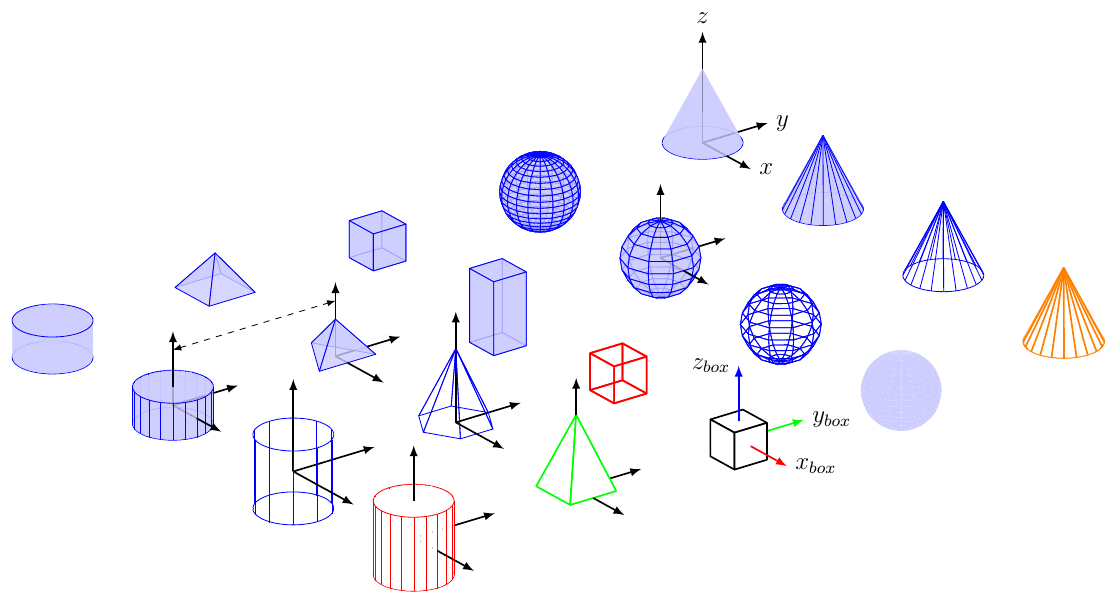
\includegraphics[width=0.7\textwidth]{chapter3/images/basic-shapes.png}
	\caption{ภาพตัวอย่างการวาดออฟเจ็คต่างๆ}
	\label{fig:basic-shapes_sk}
\end{figure}
\begin{figure}[htbp]
	\centering
	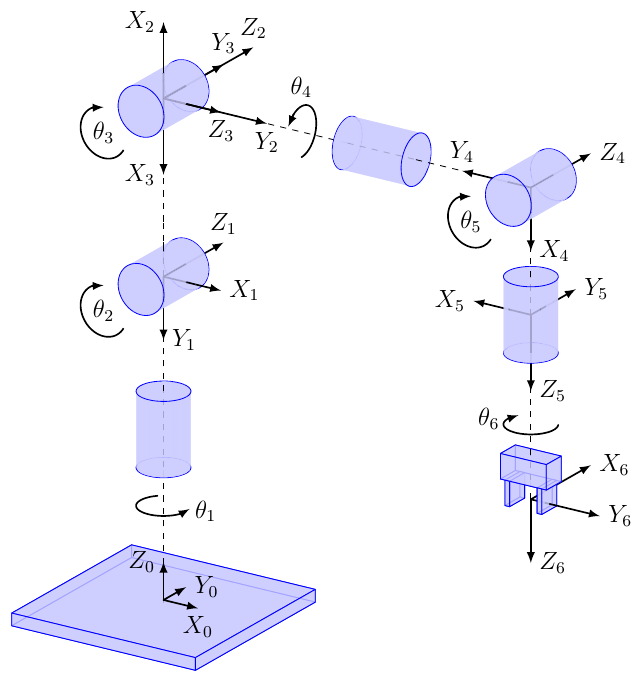
\includegraphics[width=0.5\textwidth]{chapter3/images/test_robot.png}
	\caption{ภาพตัวอย่างการวาดเฟรมของแขนกล}
	\label{fig:test-robot_sk}
\end{figure}
\begin{figure}[htbp]
	\centering
	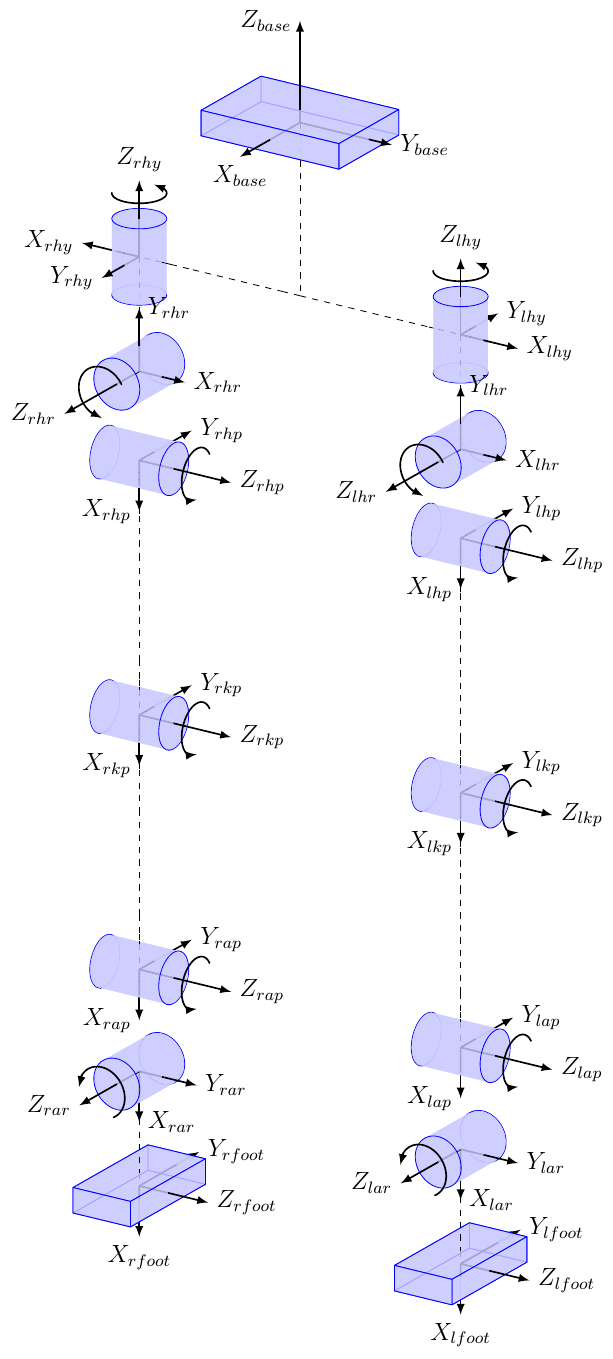
\includegraphics[width=0.4\textwidth]{chapter3/images/uthai_kinematics.png}
	\caption{ภาพตัวอย่างการวาดเฟรมของหุ่นยนต์ฮิวมานอยด์}
	\label{fig:uthai_kinematics_sk}
\end{figure}